% Created 2016-06-09 Thu 15:49
\documentclass[12pt,t,xcolor=table]{beamer}

\input{/home/stephan/H/Styles/style_presentation.tex}
\usetheme{default}
\author{Stephan Lindner}
\date{6/7/2016}
\title{Exacloud: An Overview}
\begin{document}

\maketitle

\section{What is Exacloud? And why is it on a Linux server?}
\label{sec:orgheadline5}
\begin{frame}[c]{}
  \begin{itemize}
    \item[\bf\thesection.] \bf\insertsection
  \end{itemize}          
\end{frame}

\begin{frame}[label={sec:orgheadline1}]{What is Exacloud?}
\begin{itemize}
\item Exacloud a server run by OHSU to support large-scale, computational and data intense workflows.

\item Currently more than 35 Terabytes of memory and more than 750 Terabytes of usable storage.

\item Housed at the Data Center at OHSU's West Campus.
\end{itemize}

\vspace{1em}
\begin{center}
  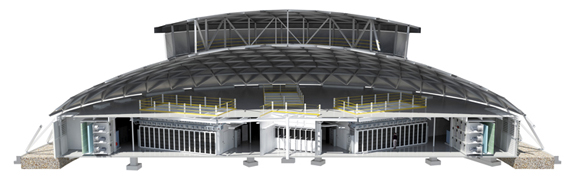
\includegraphics[width=.8\textwidth]{Figures/ohsu-datacenter.png}
\end{center}
\end{frame}



\begin{frame}[label={sec:orgheadline2}]{Exacloud and Linux}
\begin{itemize}
\item Exacloud uses Linux as operating system.

\item By contrast, the CHSE server (and our computers) use Windows as operating systems.

\item An operating systems is the ``habitat of your programs'' --- the software that manages a computer's basic functioning.

\item Linux and Windows get along OK, but they do not particularly like each other.

\item Most programs (such as R, stata) are developed for both OS (and Mac's OS).
\end{itemize}
\end{frame}

\begin{frame}[label={sec:orgheadline3}]{Why does Exacloud uses Linux?}
Linux is \ldots{}

\begin{itemize}
\item Very stable.

\item Slim and scalable and therefore has less hardware requirements.

\item Designed as a multi-user system.

\item More secure than Windows.

\item FOSS (Free and Open Source Software).
\end{itemize}
\end{frame}

\begin{frame}[label={sec:orgheadline4}]{What does this mean for us:}
\begin{itemize}
\item Most programs we use for our analysis are open-source and are developed on Linux: R, git, markdown.

\item Stata is more geared toward Windows but has some Linux support.

\item Interaction between local Windows machines and a Linux server are not perfect but fine.
\end{itemize}
\end{frame}

\section{Accessing and navigating Exacloud}
\label{sec:orgheadline9}
\begin{frame}[c]{}
  \begin{itemize}
    \item[\bf\thesection.] \bf\insertsection
  \end{itemize}          
\end{frame}

\begin{frame}[label={sec:orgheadline6}]{Accessing Exacloud via ssh}
\begin{itemize}
\item Remote access of CHSE server: through Windows desktop.

\item Remote access of Exacloud: through ssh (secure shell).

\item Shell is a command prompt that you can use to interact with the computer (e.g., run programs).

\item Bare-bone, 1970 technology that requires very little memory.
\end{itemize}
\end{frame}

\begin{frame}[fragile,label={sec:orgheadline7}]{MobaXterm: ssh for Windows}
 \begin{itemize}
\item Install MobaXterm on desktop.

\item Initiate ssh session with 
\begin{itemize}
\item Remote host: \texttt{exacloud.ohsu.edu}
\item User name: your OHSU user name.
\end{itemize}

\item Prompts for password and then connects to server.
\end{itemize}


\emph{Switch to MobaXterm}
\end{frame}

\begin{frame}[fragile,label={sec:orgheadline8}]{Navigating Exacloud}
 A couple of useful commands:

\begin{itemize}
\item Printing the working directory: \texttt{pwd}

\item Listing files in current directory: \texttt{ls (-lh / -a)}

\item Start R: \texttt{R}

\item Start stata: \texttt{stata}

\item Check git status: \texttt{git status}

\item Work with hcondor (?): \texttt{condor\_submit}, \texttt{condor\_q}
\end{itemize}
\end{frame}
\section{Using hcondor on Exacloud}
\label{sec:orgheadline10}
\begin{frame}[c]{}
  \begin{itemize}
    \item[\bf\thesection.] \bf\insertsection
  \end{itemize}          
\end{frame}
\end{document}